\documentclass{standalone}

\usepackage{tikz}
\usetikzlibrary{arrows.meta}
\tikzset{%%
  >={To[length=2.5pt]}
  }

\definecolor{myBlue}{RGB}{56, 77, 193}

  
\begin{document}
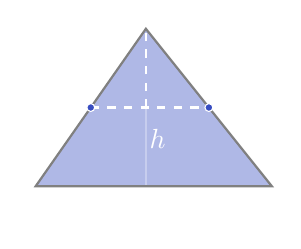
\begin{tikzpicture}
  \fill[fill=myBlue, opacity=0.4] (0,0)--(3,0)--(1.4,2);
  \node[white] at (2,-0.2) {$ b $};
  \draw[thick,white,opacity=0.3] (1.4,1)--(1.4,0);
  \node[white] at (1.55,0.6) {$ h $};
  \draw[white, thick, dashed] (0.7,1)--(2.2,1);
  \draw[white, thick, dashed] (1.4,1)--(1.4,2);
  \draw[white, ->,thick] (2,1.5) to [bend left=45] (2.8,0.5);
  \draw[white, ->,thick] (0.8,1.5) to [bend right=45] (0,0.5);
  %\draw[double, ->,thick] (3.05,0.6) to  (3.5,0.6);
  \draw[color=gray,thick,opacity=1] (0,0)--(3,0)--(1.4,2)--(0,0)--(3,0);
  \draw[white, fill=myBlue] (0.7,1) circle (0.05);
  \draw[white, fill=myBlue] (2.2,1) circle (0.05);
\end{tikzpicture}
\end{document}